% RESULTS


We still need the following:
% list
\begin{itemize}
    \item images of alingment marks
    \item IES test of LED. I-V curve
\end{itemize}


Results we will list:

\begin{enumerate}
    \item undercut in SEM image (done)
    \item alignment accuracy
    \item etch debth for GaAs etch
    \item etch debth for AlGaAs etch
    \item PECVD Si3N4 thickness vs. deposition time, reflection curve vs. wavelength (or at least the reflection minima for the final thickness and the reflectivity at 675 nm).
    \item Optical images of the sample after finishing steps in the PECVD independent work.
    \item Optical image of final LED
\end{enumerate}


% figure Undercut_5min_1200mJcm-2.jpg
\begin{figure}[ht]
    \centering
    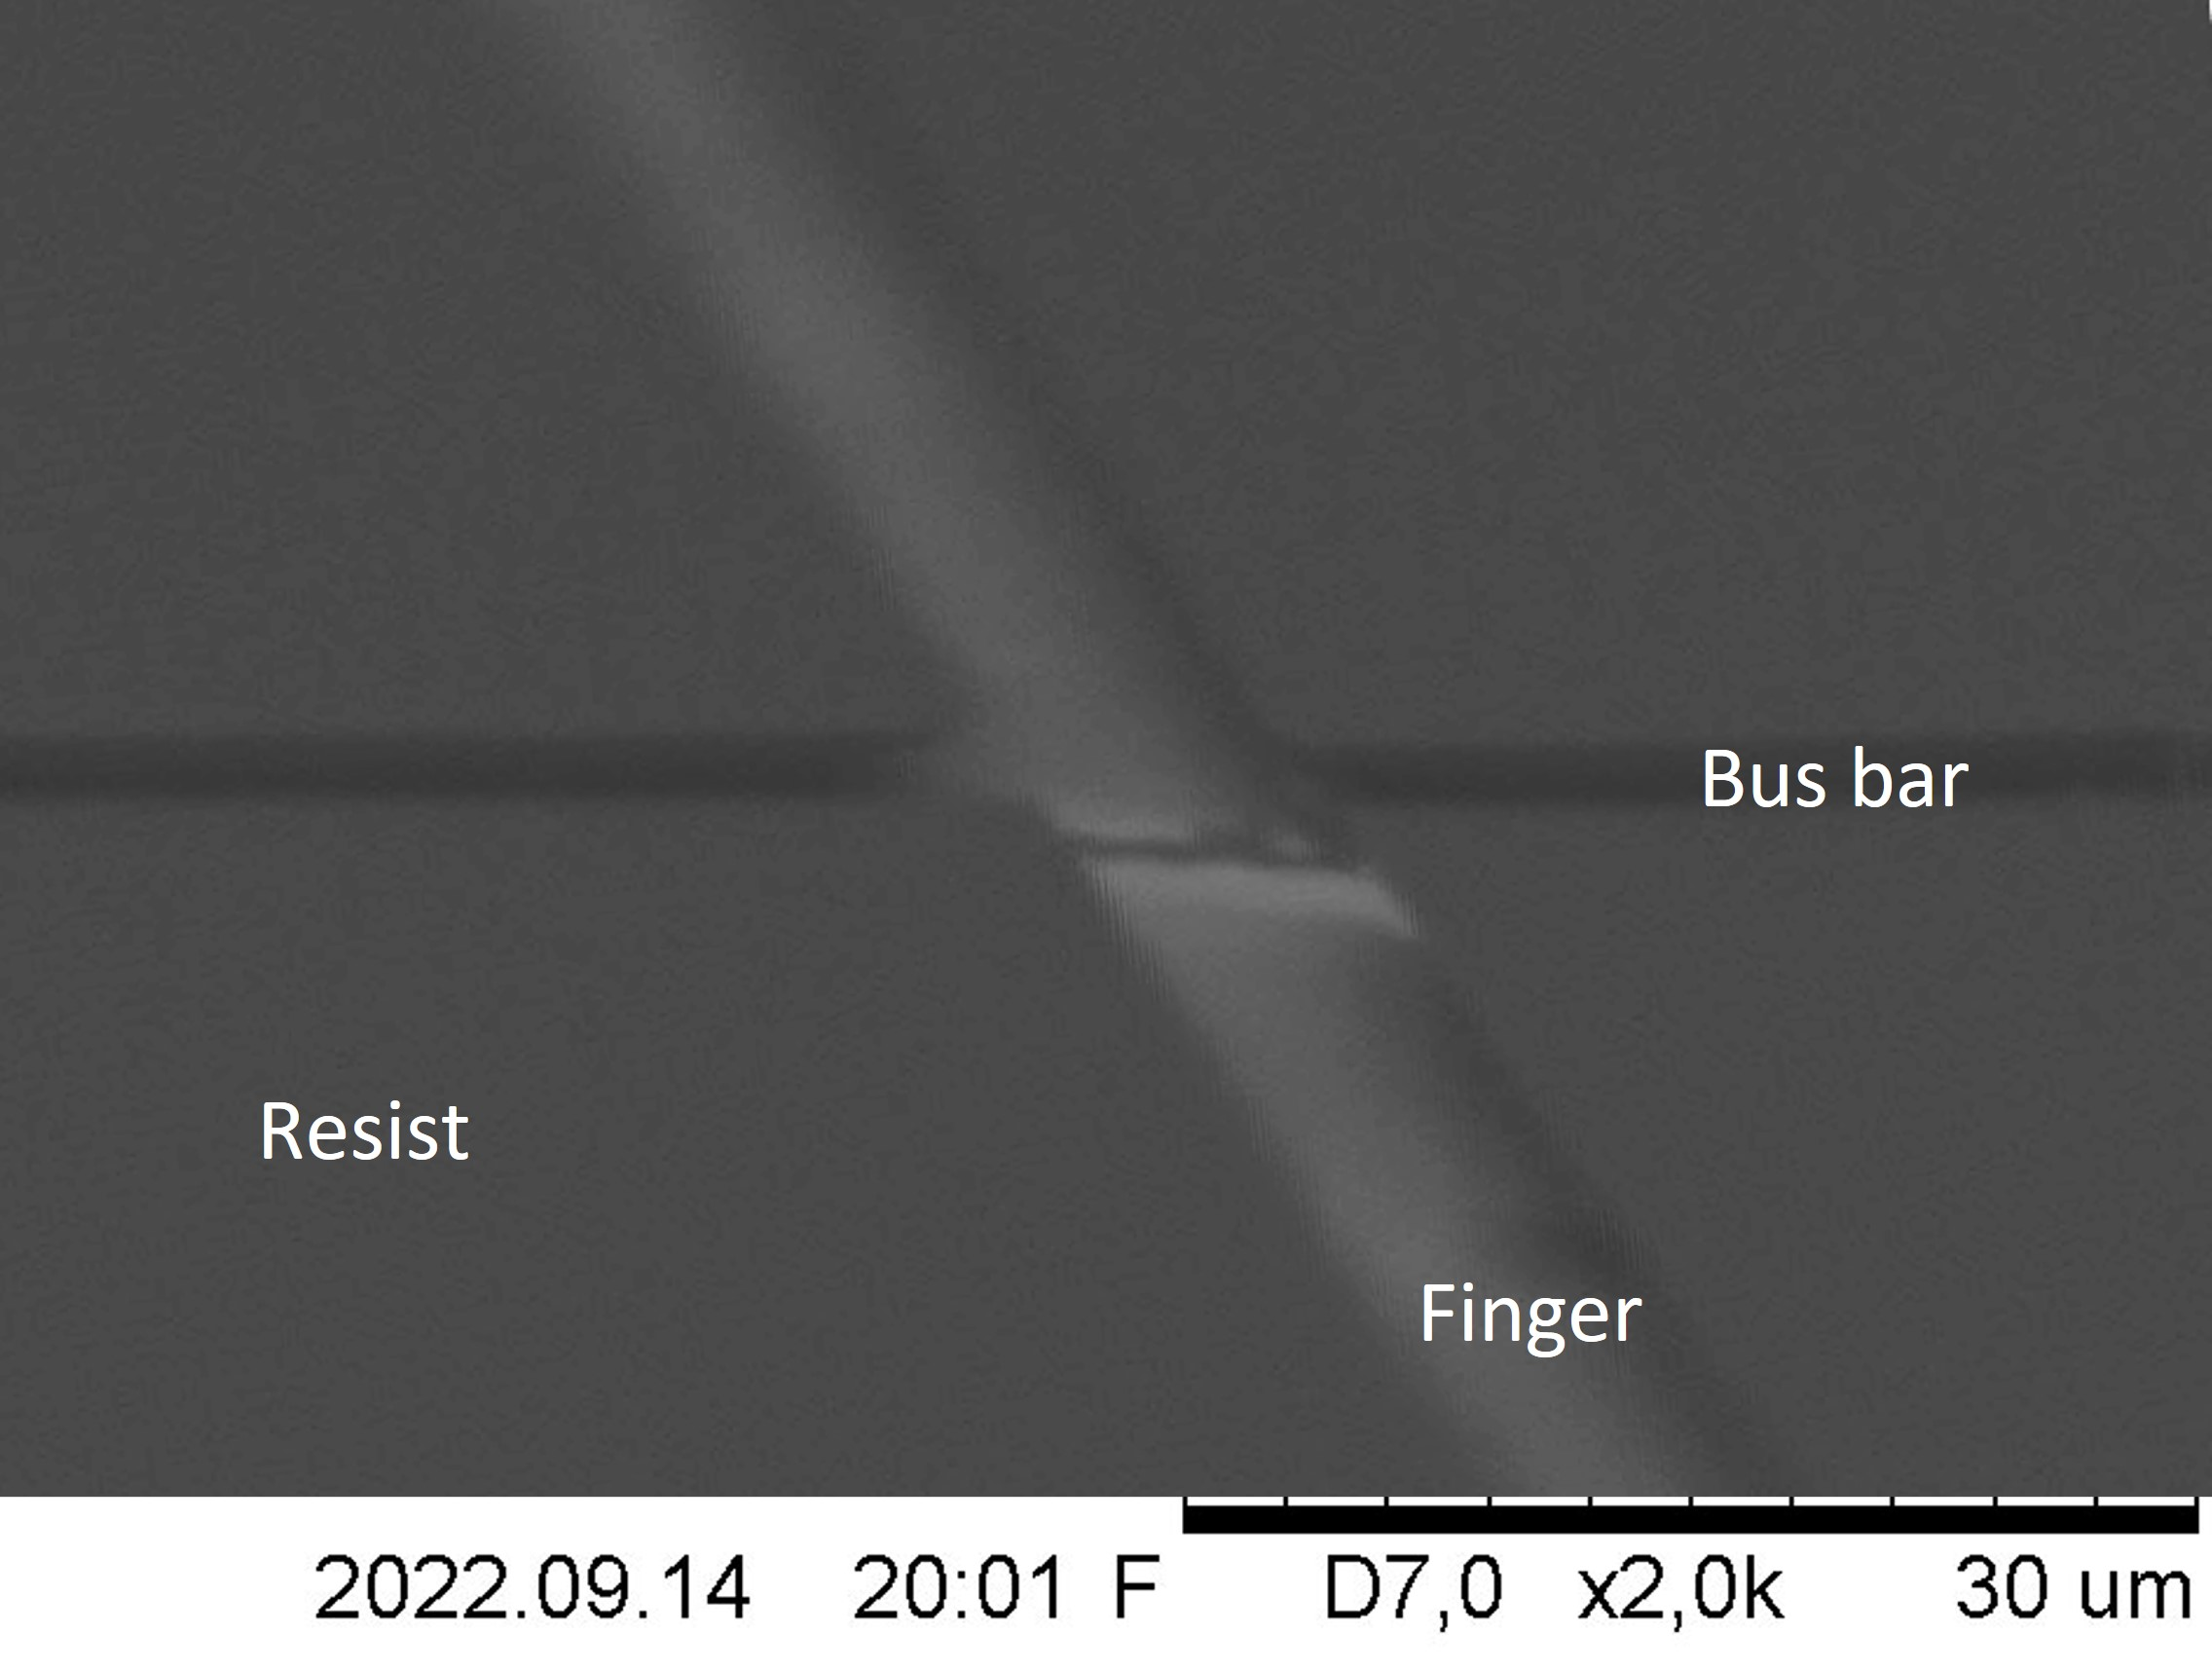
\includegraphics[width=0.45\textwidth]{figures/Undercut_5min_1200mJcm-2.jpg}
    \caption{
        SE SEM image of the undercut in the dose test.
        The optimal dose was 1300 mJ/cm$^2$ and the optimal developing time was 5 min.
        The students were not able to measure the excact undercut, but from the image it seems to be around 1 \textmu m.
        It is hard to determine the exact undercut from the image, because of the focus, the tilt and the debth in the image.
        However, it is clear that the given dose and developer time is sufficient to achieve an undercut.
        Acceleration voltage in the SE image was 5 kV.
        SEM image taken at the Hitachi TM3000 table top SEM at NTNU NanoLab.
    }
    \label{fig:undercut}
\end{figure}